% mainfile: ../../../../master.tex
\subsection{Filtering seawater on Sterivex\texttrademark~ filters for metagenomic studies}
% The part of the label after the colon must match the file name. Otherwise,
% conditional compilation based on task labels does NOT work.
\label{task:20180306_cj0}
\tags{lab,svx,sb}
\authors{cj}
%\files{}
%\persons{}

I started the filtration of the metagenomic stations at 9:00 AM with \texttt{SB5 0m} (surface), \texttt{SB5 bottom}, and \texttt{SB2 bottom} and finally \texttt{SB2 0m} (surface).

I noticed that there was slighly less water for \texttt{SB2 0m}.

\comment{It was a little hard to work today because I was on my periods.}

\comment{Anouk is busy with Alex and Sigurlaug organising the samples in the freezers.}

\comment{I also took the time to partially record the filtering process with the GoPro so in case someone else has to go on the ship or do the filtration later, it will be a useful ressource.}

\comment{I talked to Biljana from Marinox about the new organisation of the teaching lab.}

There is definitely one copepod in the Sterivex filter for station \texttt{SB5 0m}.

\begin{figure}[H] % position of the figure 
    \centering
    \caption{Pictures of the filtration process}
    \label{fig:label}
    \begin{subfigure}[b]{0.49\textwidth}
        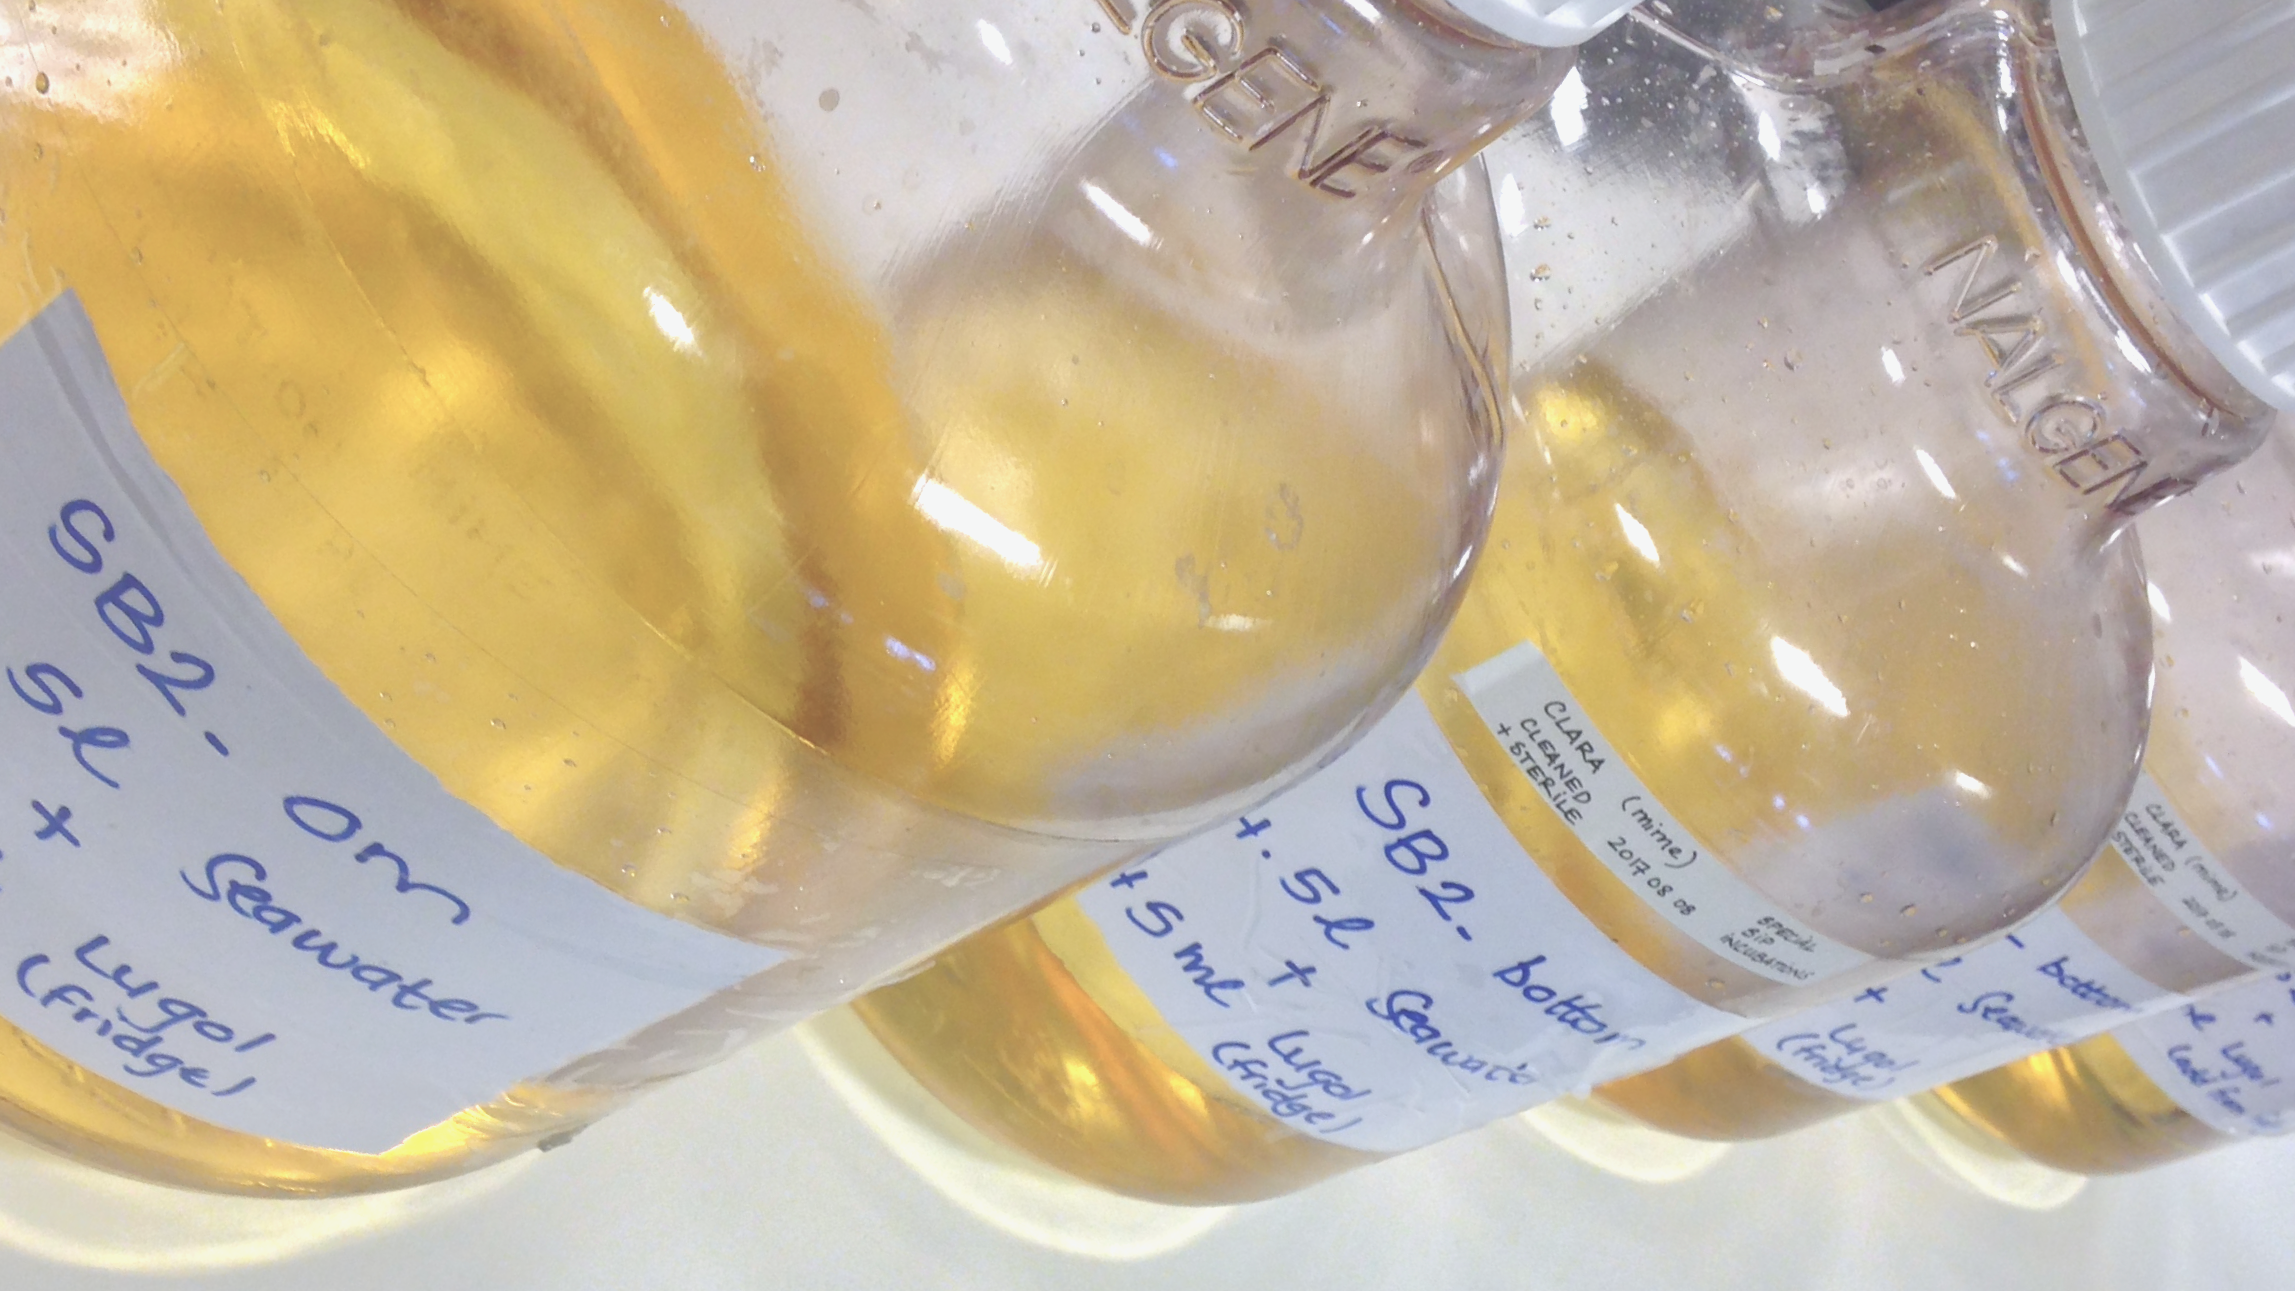
\includegraphics[width=\textwidth]{graphics/pic/20180306_seawater_samples.png}
        \caption{Seawater samples (4.5L) with 1\% lugol for metagenomic studies}
        \label{sfig:slabel1}
    \end{subfigure}
    ~ 
    \begin{subfigure}[b]{0.49\textwidth}
        \includegraphics[width=\textwidth]{graphics/pic/20180306_filtration_system.png}
        \caption{Homemade filtration device allowing simultaneous filtration on three Sterivex\texttrademark filters}
        \label{sfig:slabel2}
    \end{subfigure}
\end{figure}